\begin{proof}
    Обозначим за \(d = \min\limits_\gamma |\zeta - z_0| > 0\). Зафиксируем \(z \in B_R(z_0)\). Тогда
    \(\forall \zeta \in \gamma \colon \dfrac{1}{\zeta - z} = \dfrac{1}{(s-z_0) - (z-z_0)} = 
    \dfrac{1}{(s-z_0)(1- \dfrac{z-z_0}{\zeta-z_0})} = \sum\limits_{n=0}^\infty \dfrac{(z-z_0)^n}
    {(\zeta - z_0)^{n+1}}\). Домножим обе части выражение на \(\dfrac{f(\zeta)}{2\pi i}\). Тогда
    получим \(\dfrac{1}{2\pi i} \dfrac{1}{\zeta - z} = \dfrac{1}{2 \pi i}
    \sum\limits_{n=0}^\infty \dfrac{(z-z_0)^n \cdot f(\zeta)}{(\zeta - z_0)^{n+1}}\). Обозначив ряд
    за \(A\), а также \(M = \max\limits_\gamma |f(\zeta)|\), можно получить оценку \(A \le 
    \left|\dfrac{z-z_0}{d}\right|^n \cdot \dfrac{M}{d}\). При этом ряд \(\sum\limits_{n=0}^\infty
    \left|\dfrac{z-z_0}{d}\right|^n\) сходится, так как \(\dfrac{z-z_0}{d} < 1\), а значит по 
    признаку Вейерштрасса ряд в первой части сходится равномерно по \(\zeta \in \gamma\). Почленным
    интегрированием легко получить 
    \[F(z) = \dfrac{1}{2\pi i} \int\limits_\gamma \dfrac{f(\zeta)}{\zeta - z}d\zeta = 
    \sum\limits_{n=0}^\infty (\dfrac{1}{2 \pi i} \int\limits_\gamma \dfrac{f(\zeta) d\zeta}
    {(\zeta - z_0)^{n+1}})(z-z_0^n) = \sum\limits_{n=0}^\infty c_n (z-z_0)^n.\]
\end{proof}

\begin{corollary}\label{14:inf_dif_int_koshi}
    С учётом параграфа 13, можно получить что интеграл Коши бесконечно дифференцируемая функция,
    а её \(n\) производная равна 
    \[F^{(n)}(z) = \dfrac{n!}{2 \pi i} \int\limits_\gamma \dfrac{f(\zeta)}{(\zeta - z_0)^{n+1}}
    d \zeta\]
\end{corollary}


\Section{Лемма Гурса}

В этом параграфе определим прямоугольник \(\Pi = \{z = x+iy \colon a \le x \le b, \, c \le y \le 
d\}\)

\begin{statement}\label{15:gurs}
    \textbf{(Лемма Гурса).} Пусть \(f(z)\) регулярна на \(\Pi\). Тогда \(\int\limits_{\partial \Pi}
    f(z) dz = 0\).
\end{statement}

\begin{proof}
    Для доказательства достаточно доказать, что \(M = |\int\limits_{\partial \Pi}f(z) dz| = 0\).
    Во всех случах, когда будем писать интеграл по границе какого-либо прямоугольника, будем
    иметь ввиду обход против часовой стрелки.

    \begin{minipage}[c]{0.28\textwidth}
    \centering
    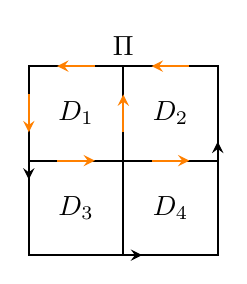
\begin{tikzpicture}[scale=1.2, >=stealth, thick]
        % Внешний прямоугольник (область П)
        \draw (0,0) rectangle (2,2);
        
        % Разделяющие крестообразные линии
        \draw (1,0) -- (1,2);
        \draw (0,1) -- (2,1);
        
        % Подписи подобластей
        \node at (0.5, 1.5) {$D_1$};
        \node at (1.5, 1.5) {$D_2$};
        \node at (0.5, 0.5) {$D_3$};
        \node at (1.5, 0.5) {$D_4$};
        
        % Подпись внешней границы П
        \node[above] at (1,2) {$\Pi$};
        
        % Стрелки обхода границы (внешние и внутренние)
        % Левая граница
        \draw[->] (0, 1.2) -- (0, 0.8);
        % Правая граница
        \draw[->] (2, 0.8) -- (2, 1.2);
        % Нижняя граница
        \draw[->] (0.8, 0) -- (1.2, 0);
        
        % Оранжевые стрелки внутреннего/поподластного обхода
        \draw[orange, ->] (0.3, 1) -- (0.7, 1);
        \draw[orange, ->] (1.3, 1) -- (1.7, 1);
        \draw[orange, ->] (0.7, 2) -- (0.3, 2);
        \draw[orange, ->] (1.7, 2) -- (1.3, 2);
        \draw[orange, ->] (1, 1.3) -- (1, 1.7);
        \draw[orange, ->] (0, 1.7) -- (0, 1.3);
    \end{tikzpicture}
\end{minipage}%
\hfill
\begin{minipage}[c]{0.70\textwidth}
    \(\int\limits_{\partial\Pi} fdz = \sum_{k=1}^{4} \int\limits_{\partial D_k} fdz.\)
    По неравенству треугольника \(M \le \sum_{k=1}^{4} \left|\int\limits_{\partial D_k} fdz\right|\)
    А значит \(\exists k : \left| \int\limits_{\partial D_k} f\,dz \right| \ge \frac{M}{4}.\)
    Обозначим такой прямоугольник за \(\Pi_1\). Исходный же прямоугольник обозначим за \(\Pi_0\).
    Аналогично деля прямоугольник \(\Pi_1\), найдём прямоугольник \(\Pi_2\) для которого выполняется
    \( \left| \int\limits_{\partial \Pi_2} f\,dz \right| \ge \frac{M}{4^2}\).
\end{minipage}
    Построим последовательность \(\Pi_1, \Pi_2, \dots \Pi_n, \dots \colon \, \left| 
    \int\limits_{\partial \Pi_n} f\,dz \right| \ge \frac{M}{4^n}\). По теореме о последовательности 
    вложенных компактов \(\exists ! \, z_0 \in \bigcap\limits_{k=0}^\infty \Pi_k\). В силу 
    дифференцируемости \(f(z)\) в точке \(z_0\) \(\exists B_\delta (z_0)\), в котором верно
    представление \(f(z) = f(z_0) + f'(z_0)(z-z_0) + \alpha(z)|z-z_0|\), где \(\alpha \in C(z_0)\)
    (вообще говоря \(\alpha(z) \in C(B_\delta(z_0))\)) и \(\alpha(0) = 0\). Теперь зафиксируем 
    \(\epsilon > 0\) и под него подберём \(\delta > 0\) такое, что \(f(z)\) регулярна в \(B_\delta
    (z_0)\) и \(\forall z \in B_\delta(z_0) \rightarrow |\alpha(z)| < \epsilon\). При известном
    \(\delta > 0\) выберем \(n \in \N\) такое, что диагональ \(\Pi_n\) \(\dfrac{d}{2^n} < \delta\) 
    (здесь \(d\)~--- диагональ прямоугльника \(\Pi_0\)). Тогда \(\Pi_n \subset B_\delta (z_0)\).
    \(\int\limits_{\partial \Pi_n} = f dz = \int\limits_{\partial \Pi_n} [f(z_0) + f'(z_0)(z-z_0)]
    dz + \int\limits_{\partial \Pi_n} \alpha(z)|z-z_0|dz\). Первый интеграл равен нулю, так как 
    подынтегральная имеет производную (например \(f(z_0)z + f'(z_0)\dfrac{(z-z_0)^2}{2}\)).
    Тогда \(\dfrac{M}{4^n} \le \left|\int\limits_{\partial \Pi_n} f(z) dz\right| \le 
    \left|\int\limits_{\partial \Pi_n} \alpha(z)(z-z_0)dz\right| \le \max\limits_{\partial \Pi_n}
    |\alpha(z)(z-z_0)| l(\partial \Pi_n) \le \epsilon \dfrac{d}{2^n} \cdot 4 \dfrac{d}{2^n}\).
    Тогда \(\dfrac{M}{4^n} \le \dfrac{4\epsilon d^2}{4^n}\), а значит \(0 \le M \le 4d^2\epsilon\).
    В силу произвольности \(\epsilon\) \(M = 0\).
\end{proof}


\Section{Интегральная формула Коши для прямоугольной области. Бесконечная дифференцируемость 
регулярной функции}

\begin{statement}
    Пусть \(f(z)\) регулярна в \(\Pi = \{z = x+iy \colon a \le x \le b, \, c \le y \le d\}\). Тогда 
    \(\forall z \in \intc(\Pi)\) выполняется \(f(z_0) = \dfrac{1}{2 \pi i} \int\limits_{\partial
    \Pi} \dfrac{f(z)}{z-z_0} dz\) (\(*\)). Здесь обход против часовой стрелки. 
\end{statement}

\begin{proof}
    Зафиксируем \(\epsilon > 0\). В силу непрерывности \(f(z)\) \(\exists \delta > 0 \colon \, 
    \forall z \in B_\delta(z_0) \rightarrow |f(z) - f(z_0)| < \epsilon\).

\begin{center}
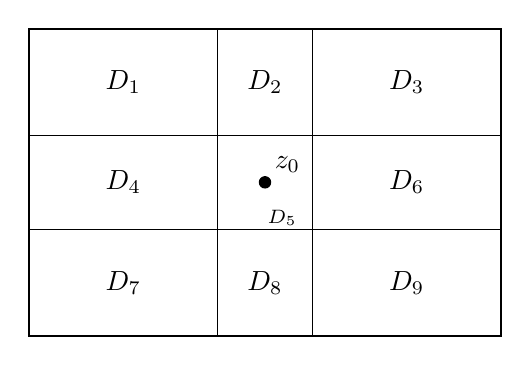
\begin{tikzpicture}[scale=1.5]

    % Внешний прямоугольник
    \draw[thick] (0,0) rectangle (4,2.6);
    
    % Центральный квадрат D5 (x: от 1.6 до 2.4, y: от 0.9 до 1.7)
    \draw (1.6,0.9) rectangle (2.4,1.7);
    
    % Вертикальные линии
    \draw (1.6,1.7) -- (1.6,2.6); % От D5 вверх (левая)
    \draw (2.4,1.7) -- (2.4,2.6); % От D5 вверх (правая)
    \draw (1.6,0)   -- (1.6,0.9); % От D5 вниз (левая)
    \draw (2.4,0)   -- (2.4,0.9); % От D5 вниз (правая)
    
    % Горизонтальные линии слева
    \draw (0,1.7) -- (1.6,1.7);
    \draw (0,0.9) -- (1.6,0.9);
    
    % Горизонтальные линии справа (продолжаются до самой правой границы)
    \draw (2.4,1.7) -- (4,1.7);
    \draw (2.4,0.9) -- (4,0.9);
    
    % Точка z_0 и подпись D5 внутри квадрата
    \fill (2.0, 1.3) circle (1.5pt);
    \node[above right] at (2.0, 1.3) {$z_0$};
    \node[below left, font=\scriptsize] at (2.35, 1.15) {$D_5$};

    % Обозначения остальных областей
    % Верхний ряд
    \node at (0.8, 2.15) {$D_1$};
    \node at (2.0, 2.15) {$D_2$};
    \node at (3.2, 2.15) {$D_3$};
    
    % Средний ряд
    \node at (0.8, 1.3) {$D_4$};
    \node at (3.2, 1.3) {$D_6$};
    
    % Нижний ряд
    \node at (0.8, 0.45) {$D_7$};
    \node at (2.0, 0.45) {$D_8$};
    \node at (3.2, 0.45) {$D_9$};

\end{tikzpicture}
\end{center}

\(D_5\)~--- квадрат со стороной \(\delta\) и центром в \(z_0\). \(\int\limits_{\partial\Pi} 
\dfrac{f(z)}{z-z_0} dz = \sum\limits_{k=1}^9 \int\limits_{\partial \Pi_k} \dfrac{f(z)}{z-z_0} dz\).
Из леммы Гурса (утверждение \ref{15:gurs}) следует, что для всех \(k\), кроме \(k = 5\), выполняется
\(\int\limits_{\partial \Pi_k} \dfrac{f(z)}{z-z_0} dz = 0\). А значит \(\int\limits_{\partial\Pi} 
\dfrac{f(z)}{z-z_0} dz = \int\limits_{\partial \Pi_5} \dfrac{f(z)}{z-z_0} dz\). Проведём оценку:
\(\left|\dfrac{1}{2 \pi i} \int\limits_{\partial\Pi} \dfrac{f(z)}{z-z_0} dz - f(z_0)\right| = 
\left|\dfrac{1}{2 \pi i} \int\limits_{\partial\Pi_5} \dfrac{f(z)}{z-z_0} dz - f(z_0)\right| = 
\left|\dfrac{1}{2 \pi i} (\int\limits_{\partial\Pi_5} \dfrac{f(z)}{z-z_0} dz - f(z_0) 
\int\limits_{\partial\Pi_5} \dfrac{dz}{z-z_0})\right| = \left|\dfrac{1}{2 \pi i} 
\int\limits_{\partial\Pi_5} \dfrac{f(z)- f(z_0)}{z-z_0} dz\right| \le \dfrac{1}{2 \pi}
\max\limits_{\partial D_5} \dfrac{f(z) - f(z_0)}{z-z_0}l(\partial D_5) \le \dfrac{1}{2 \pi} 
\dfrac{\epsilon}{\frac{\delta}{2}}4\delta = \dfrac{4}{\pi} \epsilon\). В силу произвольности 
\(\epsilon\) теорема доказана. При оценке использовался вывод из примера \ref{11:int_square}.
\end{proof}

\begin{corollary} \label{16:inf_dif_reg_func}
    Правая часть (\(*\))~--- интеграл Коши. Тогда, используя следствие \ref{14:inf_dif_int_koshi}
    получаем следующий результат: регулярная в прямоугольнике \(\Pi\) функция \(f(z)\) бесконечно
    дифференцируема в \(\intc(\Pi)\).

    В том же следствии \ref{14:inf_dif_int_koshi} приводилась формула производной интеграла Коши,
    а значит \(f^{(n)}(z) = \dfrac{n!}{2 \pi i} \int\limits_{\partial \Pi} \dfrac{f(\zeta) d\zeta}
    {(\zeta - z)^{n+1}}\).

    Обобщением данного факта является следующее: регулярная в области \(G\) функция \(f(z)\) 
    бесконечно дифференцируема в ней, так как любая точка области~--- внутренняя, а значит найдётся
    прямоугольник, полностью лежащий в \(G\).
\end{corollary}

\begin{corollary}
    \textbf{(Теорема Мореры).} Если \(f(z) \in C(G)\), где \(G\)~--- область и для любой простой
    замкнутой ломаной \(\gamma \subset G\) верно, что \(\int\limits_\gamma f(z) dz = 0\), то
    \(f\) регулярна в \(G\).
\end{corollary}

\begin{proof}
    В связи с пунктом 2) утверждения \ref{12:int_kontur} \(f(z)\) имеет первообразную в области 
    \(G\), но тогда сама первообразная \(F(z)\) регулярна в \(G\). В силу следствия 
    \ref{16:inf_dif_reg_func} \(F(z)\) принадлежит классу бесконечно дифференцируемых функций
    (обозначать будем \(F(z) \in C^\infty(G)\)). Но тогда и \(f(z)\), будучи производной её
    первообразной также принадлежит этому классу.
\end{proof}


\Section{Интегральная теорема Коши}

Здесь и далее теорема помеченные (МА)~--- теоремы, которые доказывались в курсе математического 
анализа. Их доказательство не требуется на экзамене, но они сами используются в доказательстве 
утверждений.

\begin{theorem}\label{17:ma}
    (МА). Пусть \(P(x, y), \, Q(x, y) \in C^1(G)\), где \(G \subset \R^2\)~--- односвязная область, 
    \(C^1\)~--- класс непрерывно дифференцируемых функций и \(P_y \equiv Q_x\) в \(G\). Тогда для
    любой замкнутой КНД кривой \(\gamma\) выполняется \(\int\limits_\gamma Pdx + Qdy = 0\)
\end{theorem}

\begin{theorem}
    \textbf{(Интегральная теорема Коши для односвязной области).} Пусть \(G \subset \Co\)~---
    односвязная область и \(f(z)\) регулярна в ней. Тогда для любого КНД контура \(\gamma \subset
    G\) выполняется \(\int\limits_\gamma f(z) dz = 0\).
\end{theorem}

\begin{proof}
    \(f(z) \in C^\infty(G)\). Пусть \(f(z) = u(x, y) + i v(x, y)\), тогда \(u, v \in C^\infty(G)\).
    Для любого КНД контура можно расписать \(\int\limits_\gamma f(z) dz = \int\limits_\gamma 
    udx - vdy + i\int\limits_\gamma vdx+udy\). Приняв в \ref{17:ma} \(P = u\), \(Q = -v\), а также
    использовав соотношения из утверждения \ref{9:Koshi_Riman}, получим что первый интеграл равен 0.
    Аналогично можно поступить с вторым интегралом. Таким образом, \(\int\limits_\gamma f(z) dz 
    = 0\).
\end{proof}

\begin{example}
    Односвязность области в условии теоремы существенна. Например функция \(f(z) = \dfrac{1}{z}\)
    регулярна в \(G = \Co \setminus \{0\}\), но \(\int\limits_\gamma \dfrac{dz}{z} = 2\pi i \ne 0\).
    Здесь был использовани результат из примера \ref{11:int_square}.
\end{example}